\section{Method}
\label{sec:method}

\subsection{Method Overview}

The core design choice in \method{} is to avoid prompt-text evidence injection. Instead of expressing intermediate reasoning as free-form text, the frozen VLA backbone is conditioned on a small set of learned visual evidence states. As shown in \Cref{fig:method}, \method{} first constructs a six-channel candidate evidence bank, screens out two low-utility channels, and then uses a task-adaptive router over the retained four effective channels. The routed evidence is mapped into visual states through the Visual State Composer before action decoding. Under this formulation, \thinkimg{} means that action prediction is guided by routed image-grounded states rather than by a long textual trace.

\begin{figure}[!t]
    \centering
    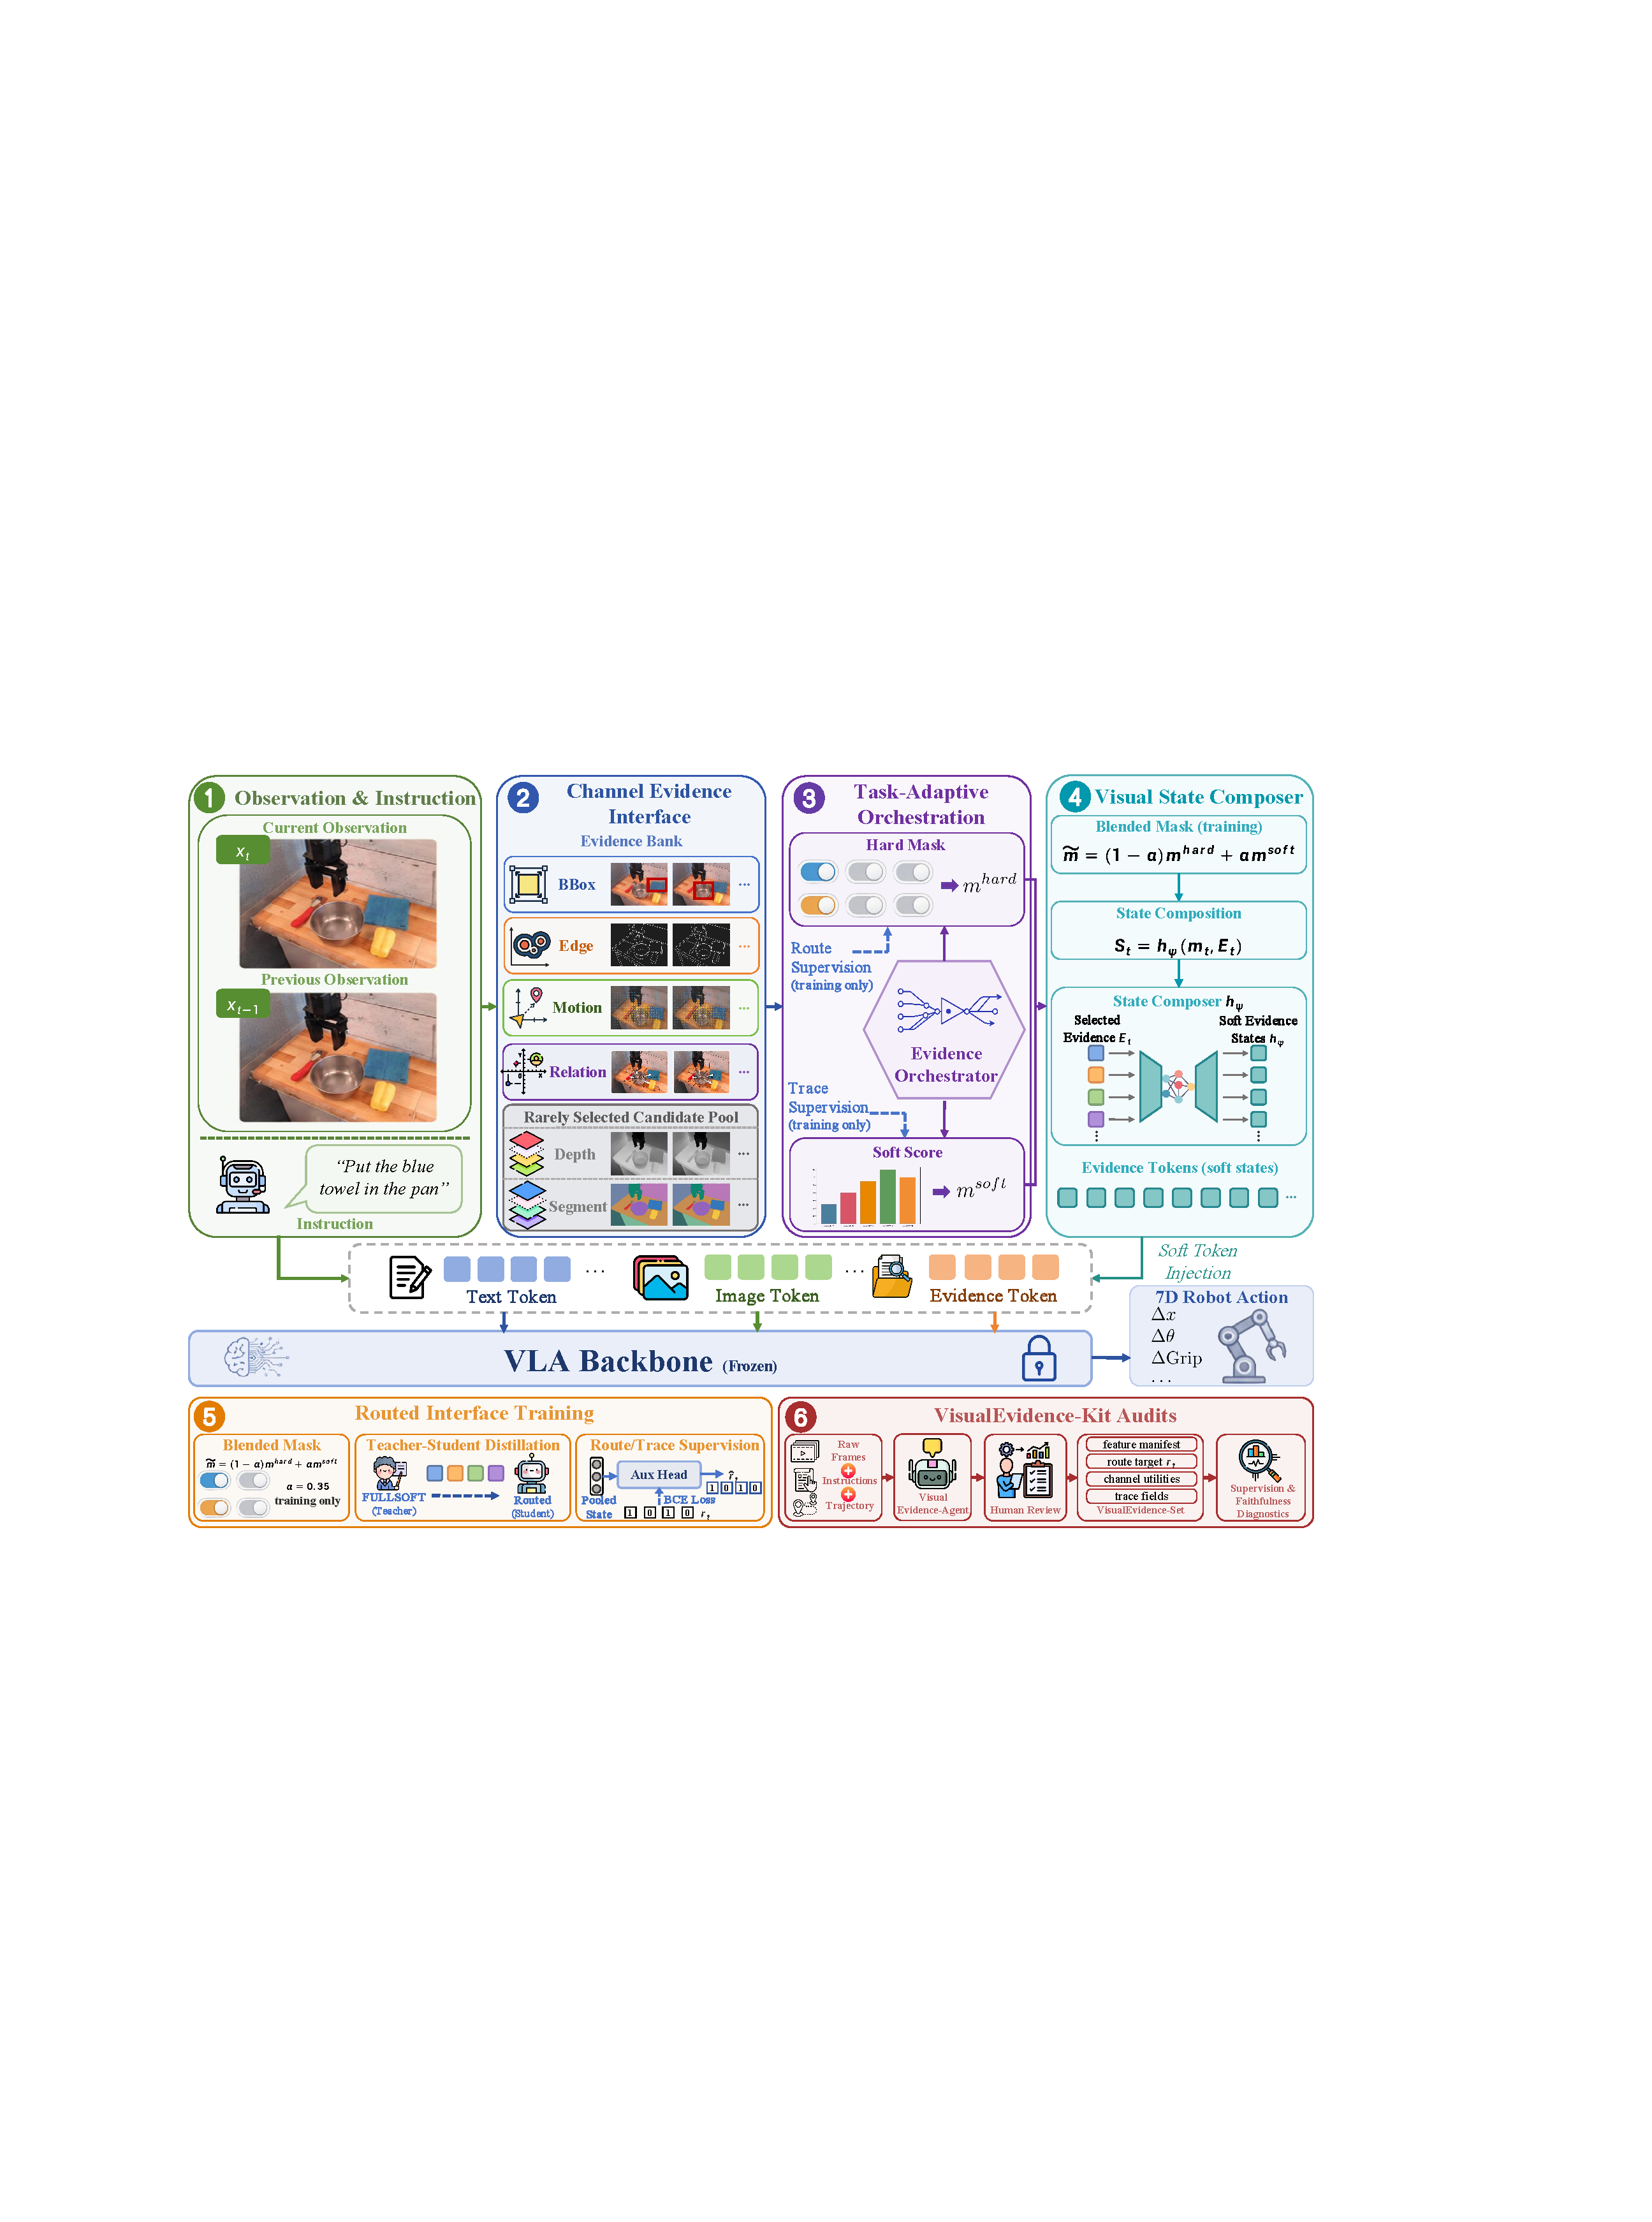
\includegraphics[width=1\textwidth]{figures/architecture.pdf}
    \caption{Overview of the \method{} pipeline. Dashed arrows denote training-only supervision.}
    \label{fig:method}
\end{figure}

\subsection{Channel Evidence Interface}
\label{subsec:soft_interface}

At decision step $t$, the policy receives the current RGB observation $x_t$, the previous observation $x_{t-1}$, and the language instruction $q$. From this context, we derive a six-channel candidate evidence bank
\begin{equation}
\mathcal{E}_t = \{e_t^{c} \mid c \in \mathcal{C}_{\mathrm{cand}}\},
\end{equation}
where
\begin{equation}
\begin{aligned}
\mathcal{C}_{\mathrm{cand}} = \{&
\texttt{bbox},\texttt{edge},\texttt{motion},\texttt{relation},\texttt{depth},\texttt{segment}\}.
\end{aligned}
\end{equation}
Each $e_t^c$ is a compact evidence vector. The construction depends on the observation pair and, for instruction-grounded channels, on $q$:
\begin{equation}
e_t^c = g_c(x_{t-1}, x_t, q).
\end{equation}
The six candidate channels cover complementary visual information: \texttt{bbox} encodes object location, \texttt{edge} captures boundary geometry, \texttt{motion} summarizes short-horizon change, \texttt{relation} represents instruction-grounded spatial relations, \texttt{depth} provides monocular geometry, and \texttt{segment} marks object regions. These channels are represented as compact vectors rather than image-sized tensors, so the VLA receives a lightweight visual interface instead of a dense auxiliary perception stack. This decomposition is aligned with recent object-centric and spatio-temporal grounding studies that separate object identity, region reference, and temporal change \citep{ravi2024sam2,yuan2025pixelrefer,yuan2025videorefer}. The detailed construction of each channel is described in the appendix.
However, channel screening identifies \texttt{depth} and \texttt{segment} as low-utility cues in our benchmark setting: they are rarely selected, bring marginal success gains, and increase side-perception overhead. We therefore define the operational evidence set and bank as
\begin{equation}
\begin{aligned}
\mathcal{C}_{\mathrm{op}} = \{&
\texttt{bbox},\texttt{edge},\texttt{motion},\texttt{relation}\}, \quad
\mathcal{E}_t^{\mathrm{op}}=\{e_t^c \mid c \in \mathcal{C}_{\mathrm{op}}\}.
\end{aligned}
\end{equation}
Accordingly, \textbf{\fullsoft{}} sets the route mask to $\mathbf{1}$ over $\mathcal{E}_t^{\mathrm{op}}$, while \textbf{\method{}} uses a router-selected sparse mask over the same four-channel bank.

\subsection{Task-Adaptive Orchestration}

A task-adaptive router predicts channel probabilities
\begin{equation}
m_t^{\mathrm{soft}} = r_{\phi}(x_{t-1}, x_t, q, \mathcal{E}_t^{\mathrm{op}}),
\end{equation}
and a hardening operator $H(\cdot)$ converts them into an inference-time route mask
\begin{equation}
m_t^{\mathrm{hard}} = H(m_t^{\mathrm{soft}}), \quad
m_t^{\mathrm{hard}} \in \{0,1\}^{|\mathcal{C}_{\mathrm{op}}|}.
\end{equation}
Given a mask $m$, we denote the routed evidence as
\begin{equation}
\mathcal{E}_t^{\mathrm{op}}(m)=\{m_{t,c}e_t^c \mid c \in \mathcal{C}_{\mathrm{op}}\}.
\end{equation}

At inference time, \method{} uses a single task-adaptive router across datasets. The hard mask $m_t^{\mathrm{hard}}$ activates only the evidence channels selected for the current decision. This is the main efficiency mechanism: all four operational channels are available to the interface, but the action decoder is exposed only to routed evidence states.

This separation also clarifies the relation among route variables. The predicted route is $m_t^{\mathrm{soft}}$, the inference-time selection is $m_t^{\mathrm{hard}}$, and the VisualEvidence-Set target $r_t$ used below is a supervised route label. The model is trained to align its predicted route with $r_t$, but at inference time it uses only its own router prediction.

\subsection{Visual State Composer}

The Visual State Composer is the concrete module denoted by $h_{\psi}$. It projects the routed channel vectors into a small set of learned visual states,
\begin{equation}
S_t = h_{\psi}(\mathcal{E}_t^{\mathrm{op}}(m)),
\end{equation}
and inserts them as conditioning states before action decoding. The frozen VLA backbone then predicts the action as
\begin{equation}
a_t = f_{\theta}(x_t, q, S_t), \quad \theta \ \text{frozen}.
\end{equation}
Because the composer consumes already-routed evidence, it adds only a lightweight learned interface; it does not invoke an online image-editing model or generate textual rationales at inference time.

\subsection{Training the Routed Interface}

Pure hard routing was brittle in difficult manipulation settings. During training, we therefore use a blended route mask
\begin{equation}
\bar m_t = (1-\alpha)m_t^{\mathrm{hard}} + \alpha m_t^{\mathrm{soft}},
\end{equation}
with $\alpha = 0.35$, and compute $S_t=h_{\psi}(\mathcal{E}_t^{\mathrm{op}}(\bar m_t))$. At inference time, $\bar m_t$ is replaced by $m_t^{\mathrm{hard}}$.

To transfer the capacity of dense evidence integration into the sparse route, we train the routed adapter with logits distillation from the four-channel \fullsoft{} teacher \citep{hinton2015distilling}. Let $p_{\mathrm{T}}^\tau$ and $p_{\mathrm{S}}^\tau$ denote teacher and student action-token distributions at temperature $\tau$. The dynamic loss is
\begin{equation}
\mathcal{L}_{\mathrm{dyn}}
= \mathcal{L}_{\mathrm{action}}
+ \lambda_{\mathrm{distill}}\tau^2
\mathrm{KL}(p_{\mathrm{T}}^\tau \Vert p_{\mathrm{S}}^\tau),
\end{equation}
with $\lambda_{\mathrm{distill}}=0.2$ and $\tau=1.5$.

VisualEvidence-Kit provides a supervised route target $r_t \in \{0,1\}^{|\mathcal{C}_{\mathrm{op}}|}$. A training-only auxiliary head predicts $\hat r_t$ from the pooled evidence state and route features. The final training objective is
\begin{equation}
\mathcal{L}_{\mathrm{total}}
= \mathcal{L}_{\mathrm{dyn}}
+ \lambda_{\mathrm{trace}}
\mathcal{L}_{\mathrm{BCE}}(\hat r_t, r_t).
\end{equation}
This route/trace supervision regularizes the evidence pathway during training; the auxiliary head and channel-grounded traces are not used at inference time.



\section{VisualEvidence-Kit}
\label{sec:visualevidence_kit}

To train and examine a policy that reasons through sparse visual evidence, we construct \textbf{VisualEvidence-Kit}, a route-grounded supervision and audit resource for VLA control. VisualEvidence-Kit contains two coupled components: a \textbf{VisualEvidence-Agent} that derives and governs evidence instructions from manipulation trajectories, and the resulting \textbf{VisualEvidence-Set} that supports route supervision and counterfactual auditing. Unlike ordinary action trajectories, its instructions explicitly describe what visual channels are relevant to the action decision and whether the routed policy depends on them. This design is also informed by data-centric learning work that uses adaptive pseudo-labeling and active annotation to handle imperfect supervision \citep{deyoung2020eraser,zhang2022boostmis}.

\begin{figure}[H]
    \centering
    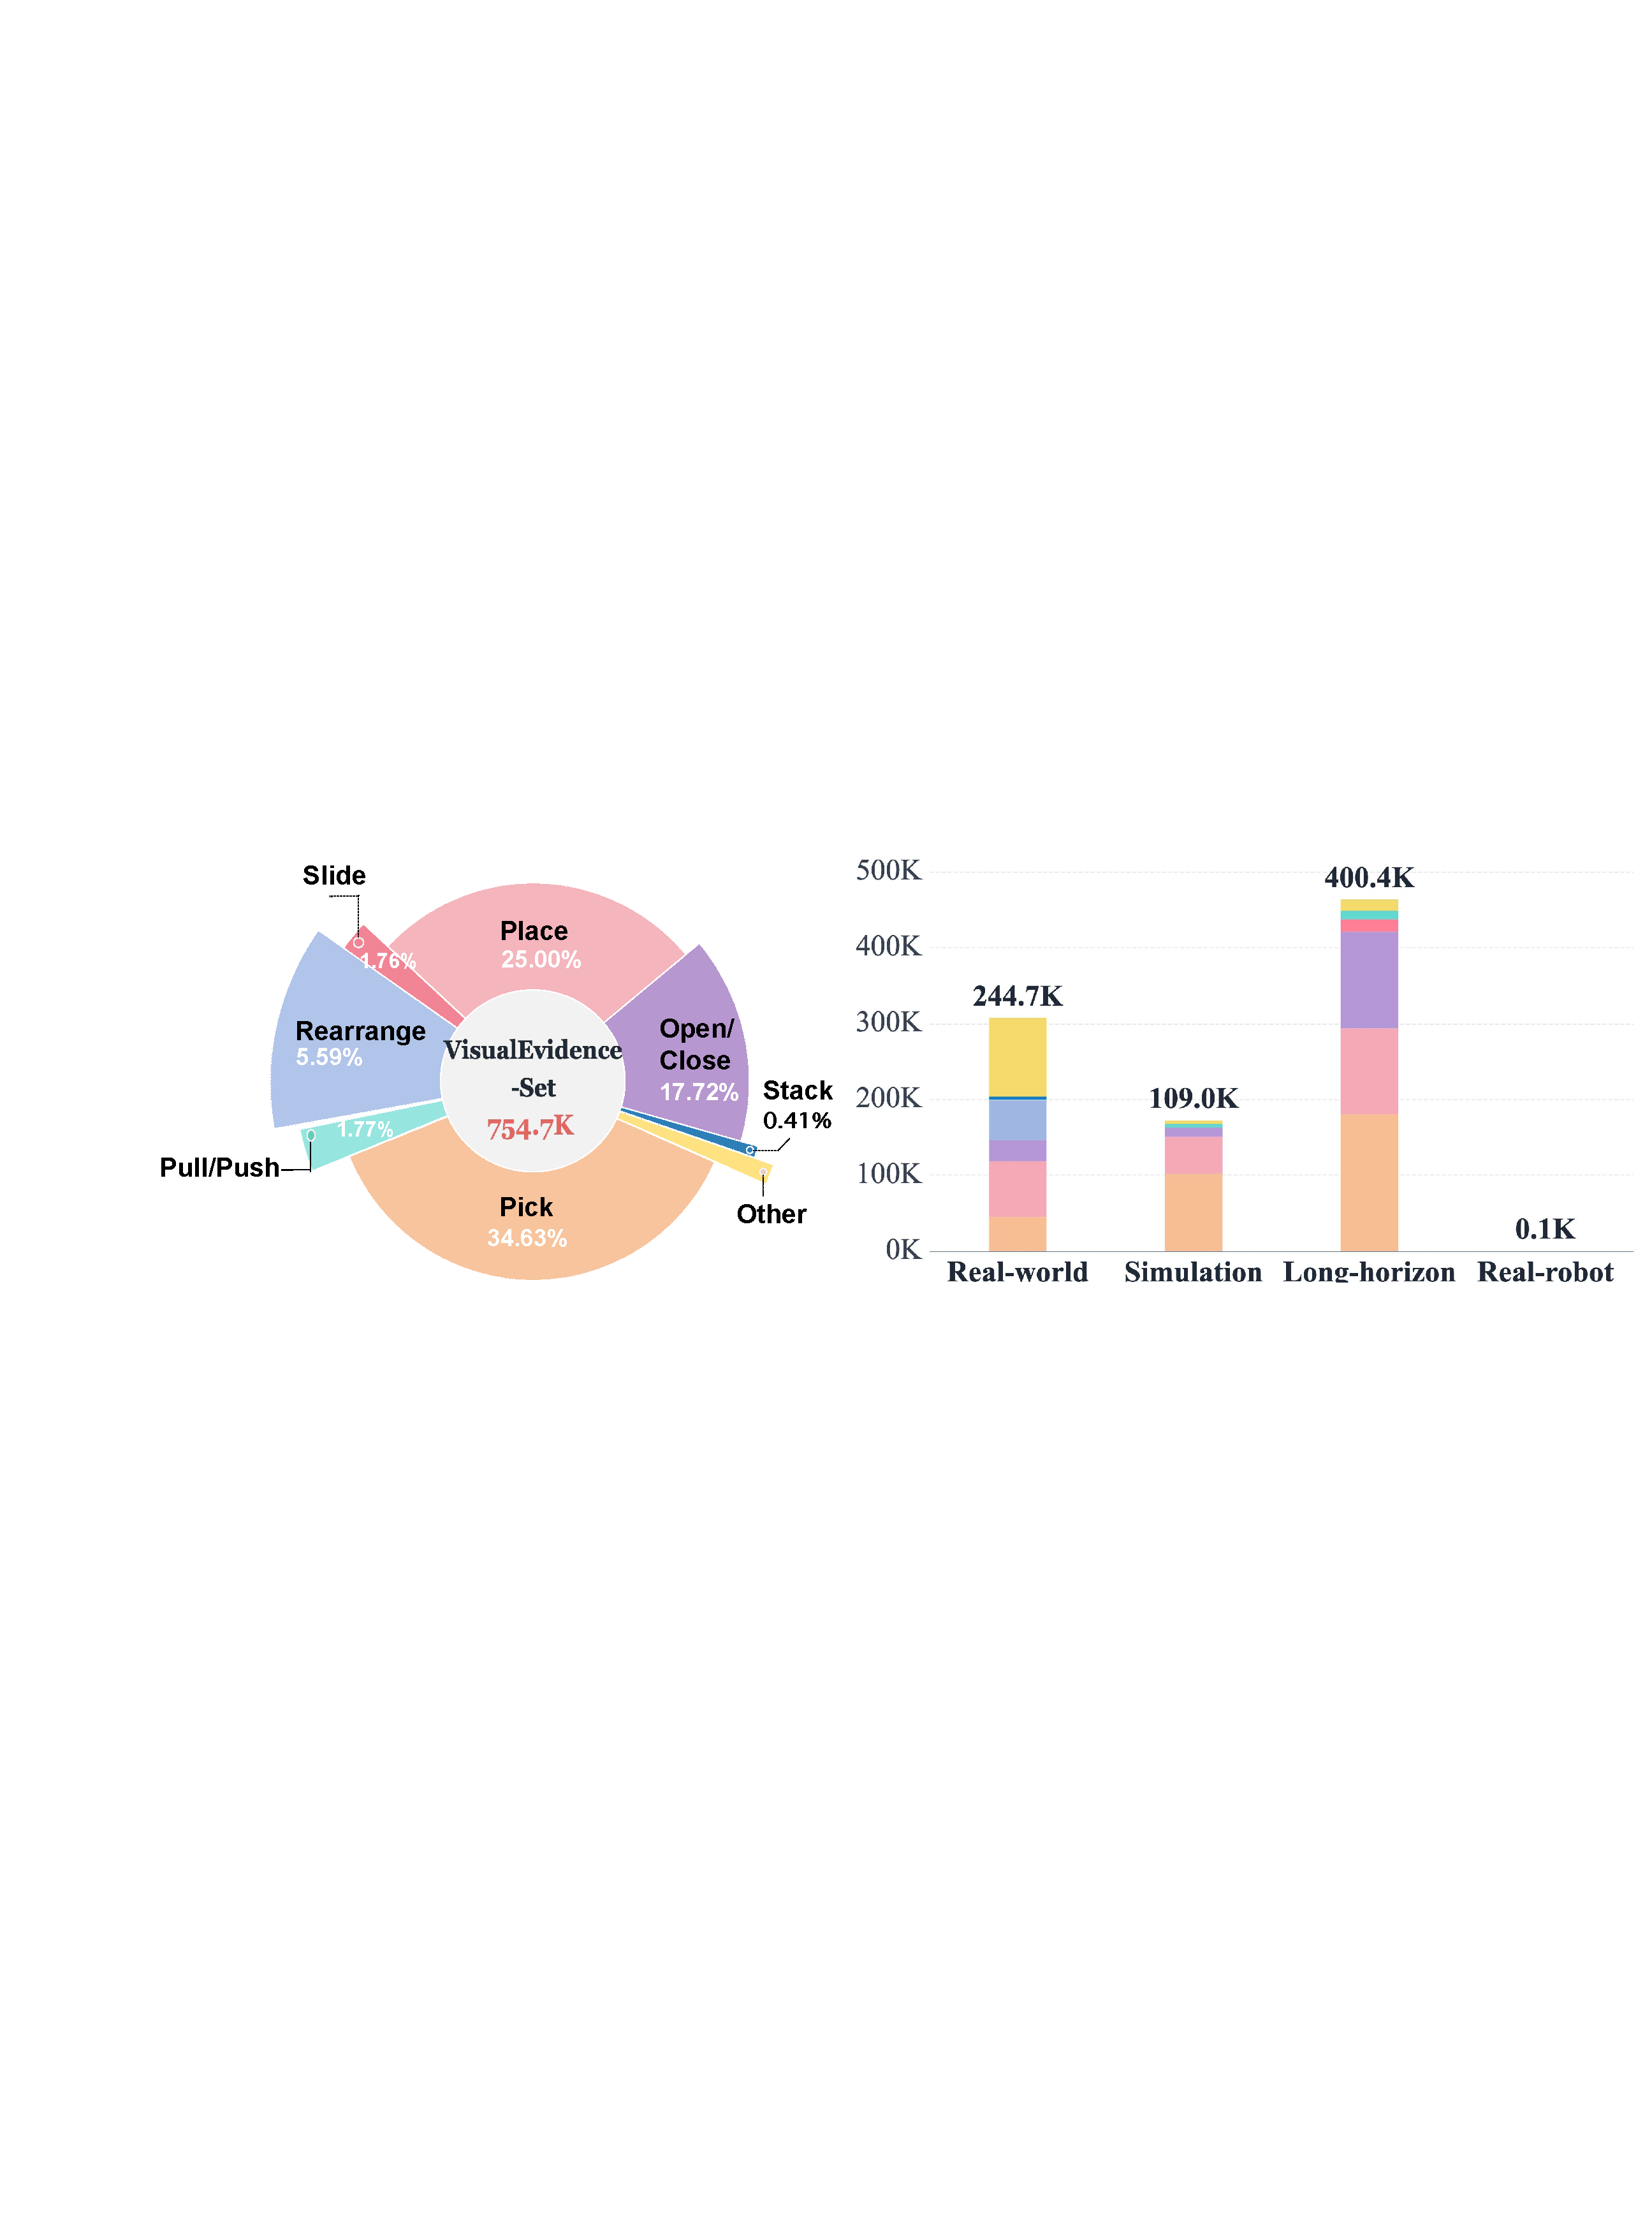
\includegraphics[width=\columnwidth]{figures/dataset-information.pdf}
    \caption{Data statistics of VisualEvidence-Set}
    \label{fig:dataset_information}
\end{figure}

\subsection{VisualEvidence-Agent}

The VisualEvidence-Agent converts raw frames and trajectory metadata into governed route-grounded instructions through four stages. 

\begin{figure}[!t]
    \centering
    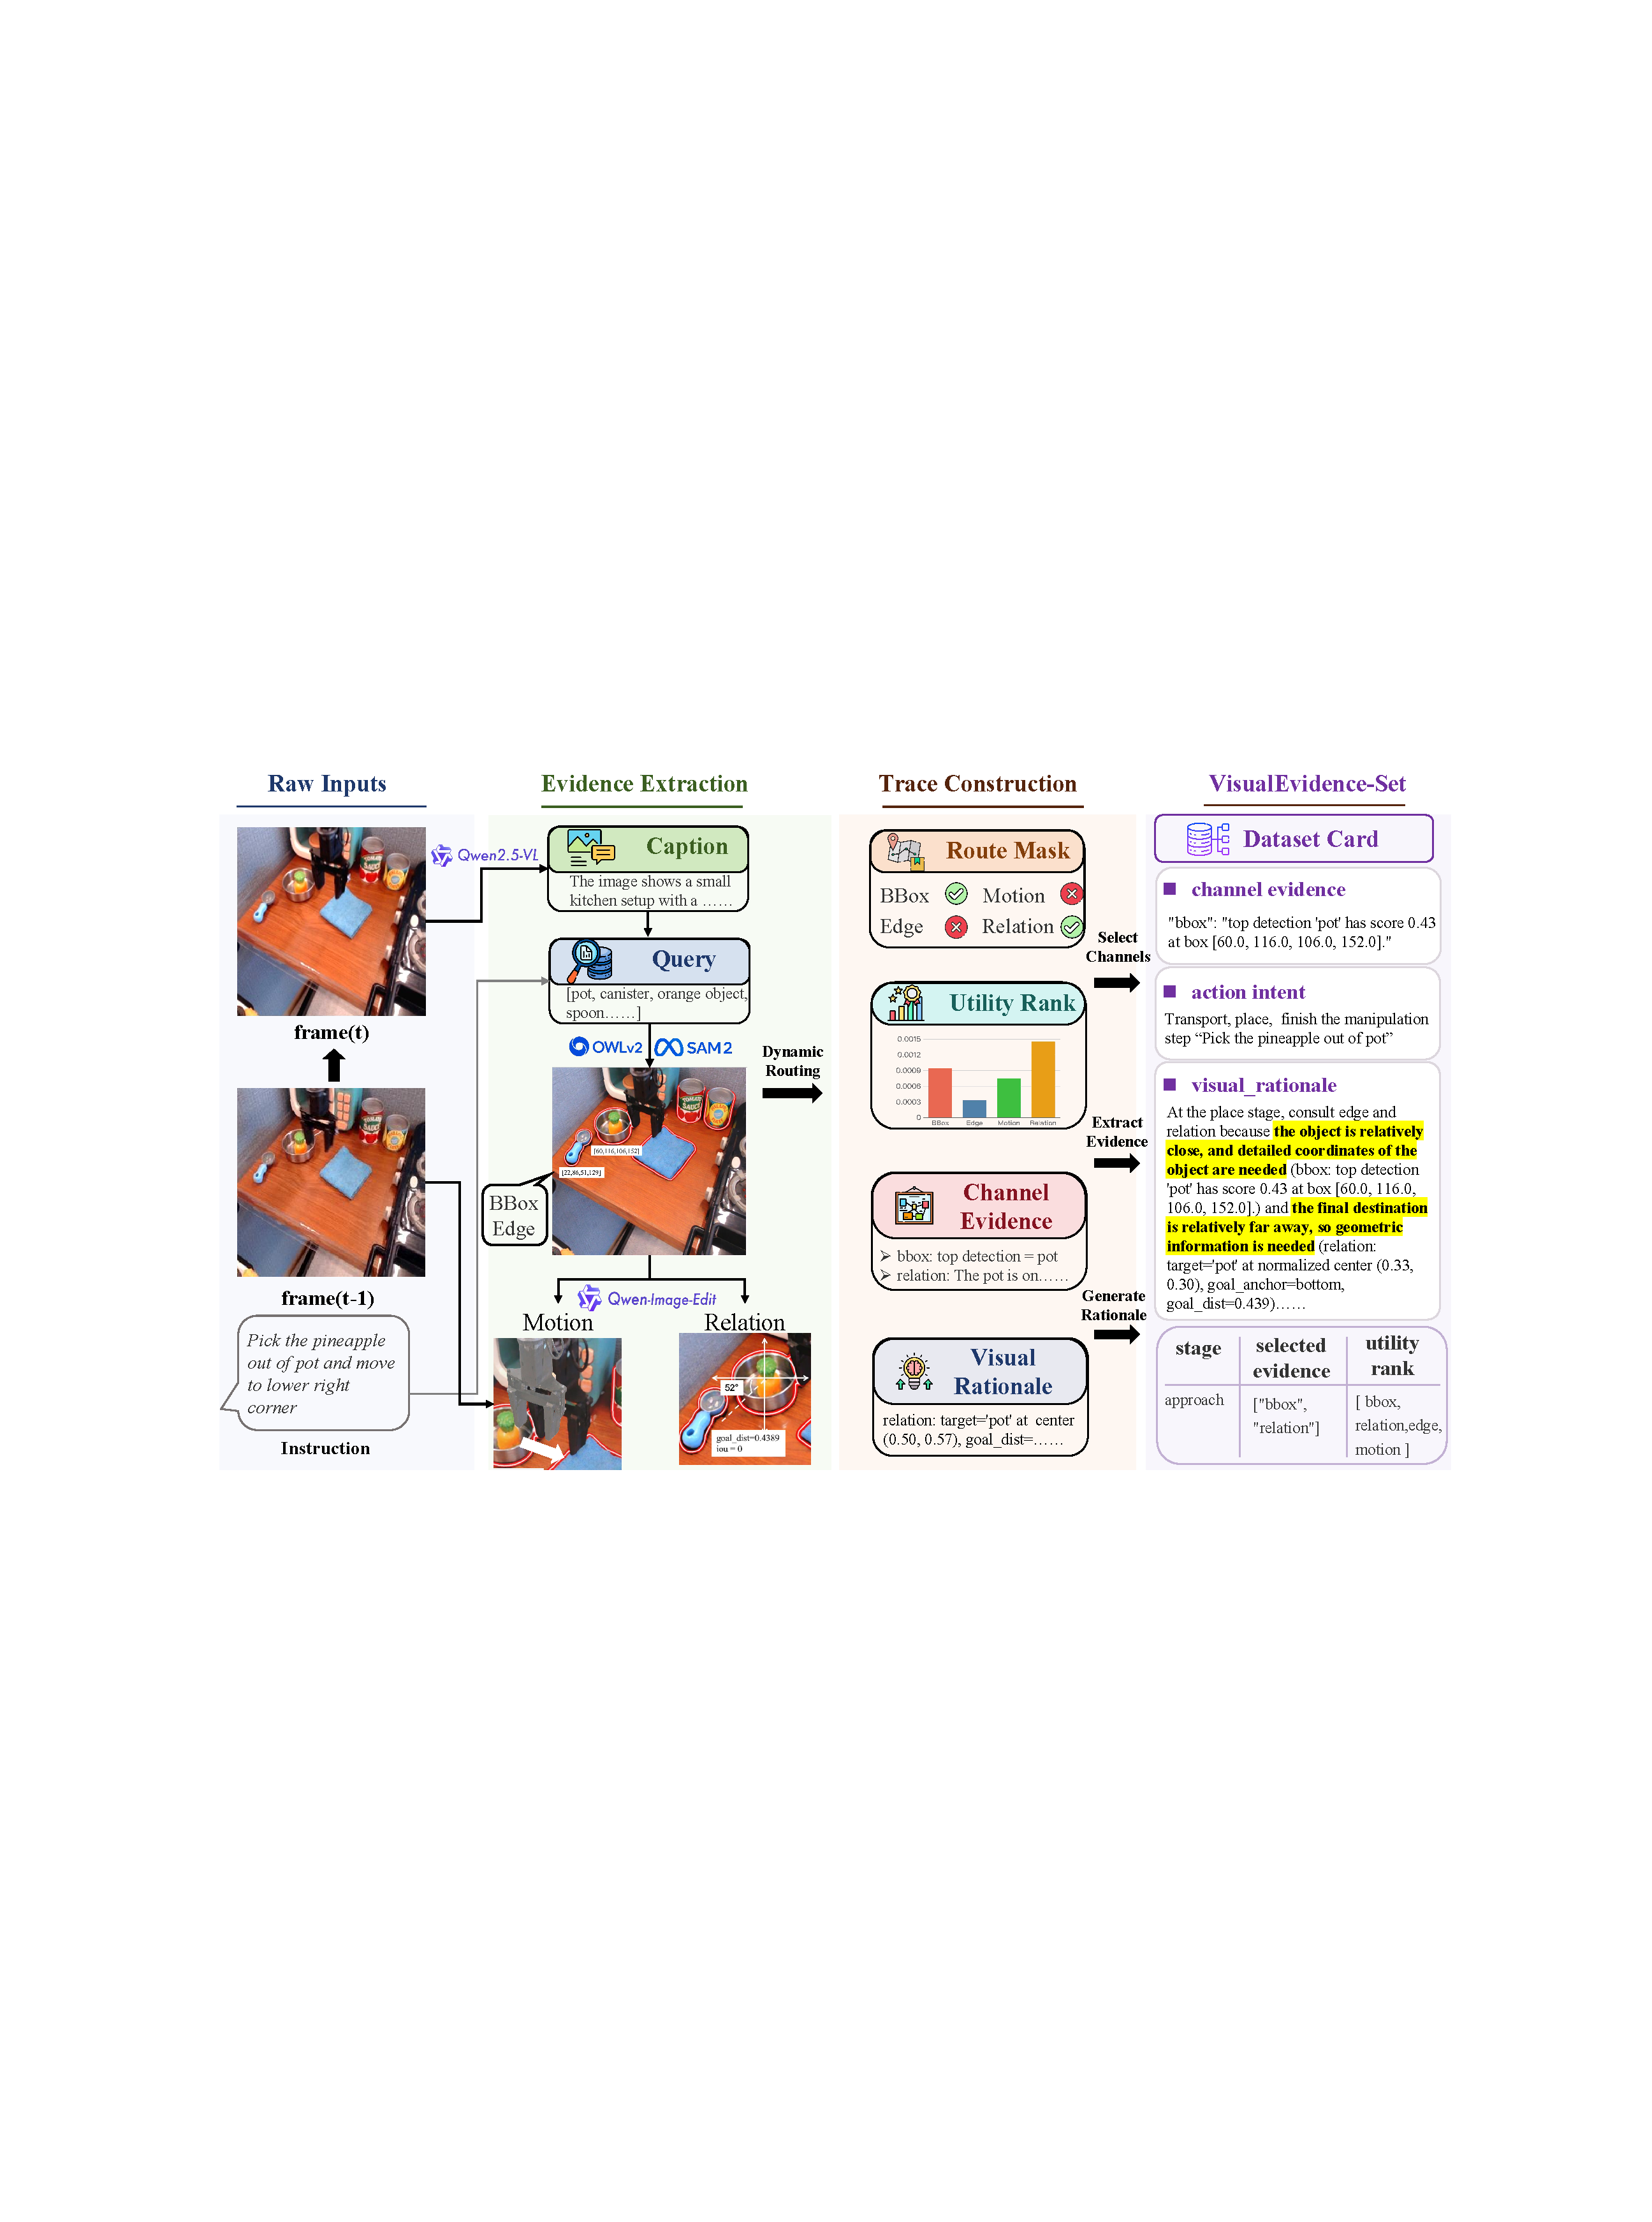
\includegraphics[width=\textwidth]{figures/visualevidence_agent.pdf}
    \caption{VisualEvidence-Kit workflow and VisualEvidence-Set record schema.}
    \label{fig:visualevidence_agent}
\end{figure}

\noindent\textit{(i) Evidence extraction}: applies the candidate channel extractors to construct a feature manifest for each decision context. 

\noindent\textit{(ii): Route and utility assessment}: aggregates routing signals and counterfactual channel utilities to form channel-level route targets and utility ranks. 

\noindent\textit{(iii): Trace construction}: records the manipulation stage, primitive, evidence dependence, difficulty, and selected evidence as a structured channel-grounded trace rather than a free-form rationale. 

\noindent\textit{(iv): Human review} verifies instruction consistency and filters unreliable labels before export. As illustrated in \Cref{fig:visualevidence_agent}, this filtering step follows the same practical concern as imperfect-label and uncertainty-aware learning: noisy supervision should be separated from high-confidence training or audit targets \citep{zhang2023learning,zhang2024revisiting}. This pipeline makes the supervision aligned with the visual interface used by \method{} while reserving the traces for training and audit only. 

\subsection{VisualEvidence-Set}

The resulting VisualEvidence-Set organizes heterogeneous manipulation information around the evidence demands of control. Each instruction contains the observation, instruction context, feature manifest, supervised route target $r_t$, counterfactual channel utilities, and channel-grounded trace fields. We further categorize the instructions along complementary axes, including scene domain, action category, manipulation stage, and routed visual evidence type, following the broader trend of heterogeneous knowledge organization in large vision-language systems \citep{qwen2025qwen25vl,lin2025healthgpt}. As summarized in \Cref{fig:dataset_information}, here displays the distribution of instructions for different action types and scene domains. In addition, each instruction is annotated by visual features, task stage, and difficulty level, enabling both router training and diagnostic evaluation across evidence requirements.

To support different use cases, we curate the constructed instructions into increasingly stringent subsets. \textit{Full-Clean} is used for corpus-level statistics and weighted training after basic consistency filtering; \textit{HQ-Trace} retains reliable structured traces for route- and trace-supervised refinement; and \textit{Gold-Faithfulness} serves as a high-reliability subset of 754.7k instructions for counterfactual audit experiments.

During policy training, VisualEvidence-Set provides route and trace supervision, while at inference time neither the agent nor its trace fields are required. For audit, we introduce counterfactual faithfulness diagnostics inspired by rationale-based and perturbation-based tests. These diagnostics evaluate whether \thinkimg{} is grounded in the policy's actually routed evidence rather than merely serving as a post-hoc explanation. The complete workflow and dataset statistics are detailed in Appendix~\ref{subsec:VisualEvidence-Kit_Workflow}.
